A streaming service can meet its delivery deadlines and still erase
usable progress. A correction selected now can become the input to later recognition
\cite{vu2026streamcorrect}. This feedback dependency creates a service
problem beyond first-delivery latency. In an actual streaming run, a
complete two-second audio interval was visible 1.44~s after it became
ready, meeting its two-second display deadline (D2). At 1.54~s, a trusted
update replaced the whole hypothesis with a shorter snapshot despite its
still-valid dependency path. Identical text returned at 3.72~s, meeting
the eight-second certified-delivery deadline (C8). Both first deliveries
were timely, yet the interval disappeared for 2.176~s
(Figure~\ref{fig:continuity_case}). We call this an \emph{avoidable
withdrawal}: an update retracts a delivered whole view that it still
supports. The client loses progress that the revision did not refute.

\begin{figure*}[t]
\centering
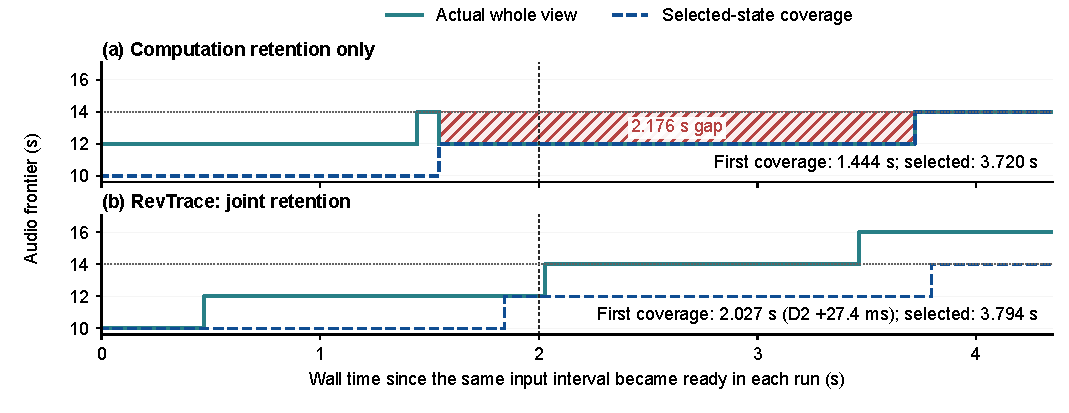
\includegraphics[width=\textwidth]{figures/timely_full_interval_case.pdf}
\caption{On-time delivery does not guarantee continued availability.
Two actual c16-overload runs process the same complete 12--14-s audio
interval using their own ready clocks. (a) Computation-only displays 37
new code points at 1.444~s, withdraws the supported view at 1.544~s and
restores identical text at 3.720~s. (b) RevTrace first displays the same
whole text at 2.027~s, missing D2 by 27.4~ms, and keeps the interval
covered thereafter. Its 3.794-s selected update retains an ahead 16-s view.
The dotted line marks D2 (2~s); both certified deliveries meet C8 (8~s).
These are separate executions with different interleavings, rather than
an event-matched counterfactual.}
\label{fig:continuity_case}
\end{figure*}

The separate RevTrace run in Figure~\ref{fig:continuity_case}(b) first
displays the same whole text slightly after D2, then retains coverage.
Its own next selected update also keeps an ahead view. The trajectories
expose first delivery and continued availability as separate obligations.

A dependable revision service must both reject invalid results and
preserve progress that remains usable. Discarding all older work enforces
a conservative boundary at the cost of service. Preserving computation
alone leaves another gap: the Consumer can still replace its valid ahead
view when a selected state installs. In a predeclared 24-speaker stratum,
computation retention improves timely audio coverage while increasing
backward movements of the displayed audio frontier, or \emph{frontier
withdrawals}, from 12 to 17. Coordinating computation and view retention
yields zero. Valid execution must therefore be connected to continued
availability at the actual Consumer.

One feedback revision can have different consequences for an executing
call, an accepted result, and a displayed hypothesis. RevTrace separates
three judgments. \textbf{[EL] Input eligibility} checks the complete frozen
input and its dependency path under the selected feedback state.
\textbf{[AU] Selection authority} keeps the original selection and ordered
installation bound to the complete original result. \textbf{[SUP] View
support} checks the Consumer's whole hypothesis when that state installs
(Figure~\ref{fig:protocol}). A call's input can be confirmed even when its
own next prediction is wrong. A view can lose support while a future
call's input is unresolved. Producer exit can end new-message authority
while leaving an already accepted result eligible. A birth version,
matching text, or producer-liveness bit cannot stand in for these
different decisions.

Dependency reuse and revocation have established foundations in
incremental dialogue and computation
\cite{schlangen2011incremental,hammer2014adapton,hammer2015names}.
SSBD coordinates draft reuse with display masking~\cite{zeng2026ssbd};
PredGen speculates across evolving speech stages~\cite{li2025predgen}.
RevTrace realizes coordination around a recursively selected feedback
task: complete calls retain the original correction and update, while
the actual whole view is checked independently at selected-state
installation. This provides a concrete use for old work without turning
a prediction into selection authority.

We make three contributions:
\begin{itemize}
\item A service contract exposing avoidable withdrawal and sufficient,
  executable witnesses for complete-call eligibility and whole-view
  support across trusted revisions
  (Sections~\ref{sec:contract}--\ref{sec:continuation}).
\item A joint coordinator that preserves the original selected transition
  relation while retaining eligible calls and supported whole views.
  Its conditional selected-trace argument connects early execution,
  durable selection and supported process failures
  (Sections~\ref{sec:continuation}--\ref{sec:protocol}).
\item Evidence that computation-only retention can worsen visible
  progress, and that confirmed full calls improve timely original-task
  service. Factorial, native and fault controls distinguish these benefits
  from text accuracy, recovery latency and load boundaries
  (Section~\ref{sec:eval}).
\end{itemize}

In the matched four-speaker native study, audio coverage meeting both
deadlines increases from 45.2\% with conservative execution to 99.2\% with
RevTrace; whole-run passes rise from zero to six of eight. A whole-run
pass meets both P99 delivery targets. The independent factorial study explains why
retaining work and retaining its delivered view are separate obligations.
